\documentclass[12pt]{article}
%	options include 12pt or 11pt or 10pt
%	classes include article, report, book, letter, thesis
\usepackage{amsmath,amsfonts,amssymb}
\usepackage{graphicx}
\graphicspath{ {images/} }

\begin{document}

\begin{titlepage}
\title{Mining Uber Dataset}
\author{Abhilash Mysore Somashekar \\Raviraj Prakash Wani \\ Satya Akhil Chowdary Kuchipudi \\Sanil Jain}
\date{1 April 2017}
\maketitle
\end{titlepage}


\textbf{Project Github Link} https://github.com/msabhi/mining-uber-dataset \break

\textbf{Objective}

The dataset collected by FiveThirtyEight contains data on over 4.5 million Uber pickups in New York City from April to September 2014. The data set is divided across six files i.e. one file per month


\textbf{Exploratory Analysis Goals}

\begin{itemize}
	\item Preprocessing of data (rounding of the Latitude and Longitudes)
	\item To find out whether 4.5 million data points over 6 months are continuous or not
	\item To plot counts in histograms as well as plot Uber pickups on actual map and look at the coverage of NYC
	\item Analyze Uber pickup data over various months
	\item Finding the hotspot locations in the data. These are the locations where there are pickups more than a specified threshold
\end{itemize}


\textbf{Graphical Analysis:} \\

 Average Pickups by Day (for all 6 months) \\
  	Comparable bars over all days of 6 months suggest that Uber data is continuous over the data set. Also similar graphs have been observed for each individual month

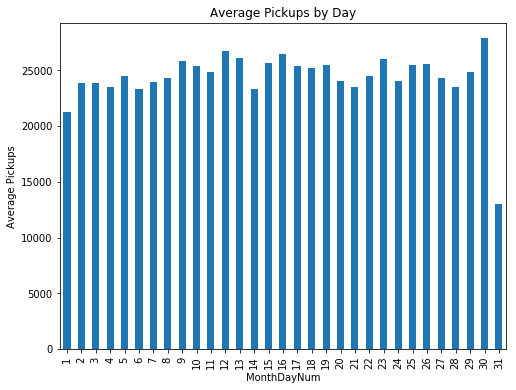
\includegraphics[width=8cm, height=8cm]{ByDay.png}

Average Pickups over a day \\
	This graph is an average of all the days data over 6 months. This suggest the evening 5:00 pm are the peak hours for Uber.

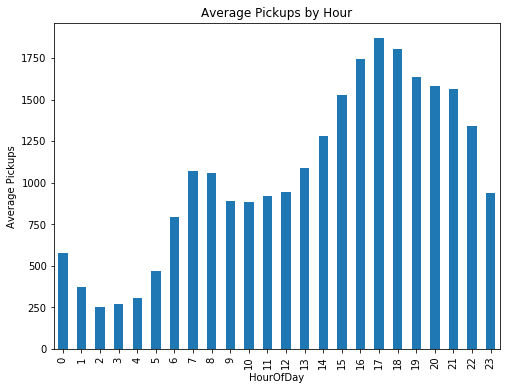
\includegraphics[width=8cm, height=8cm]{ByHour.png}	

Average Pickups over 6 months (April to September) \\
	The plot of cumulative pickups suggest that Uber business has grown over these set of months since average number of pickups have almost doubled from April to September

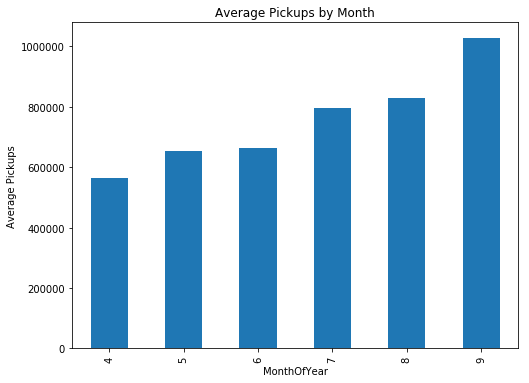
\includegraphics[width=8cm, height=8cm]{ByMonth.png}	

\textbf{Geographical Plot (Density Plot)}  \\

Plotting 4.5 million data points:
The complete density plot carves out the map of New York City on a black canvas by geography. This further strengthens the range of geographical data in dataset.

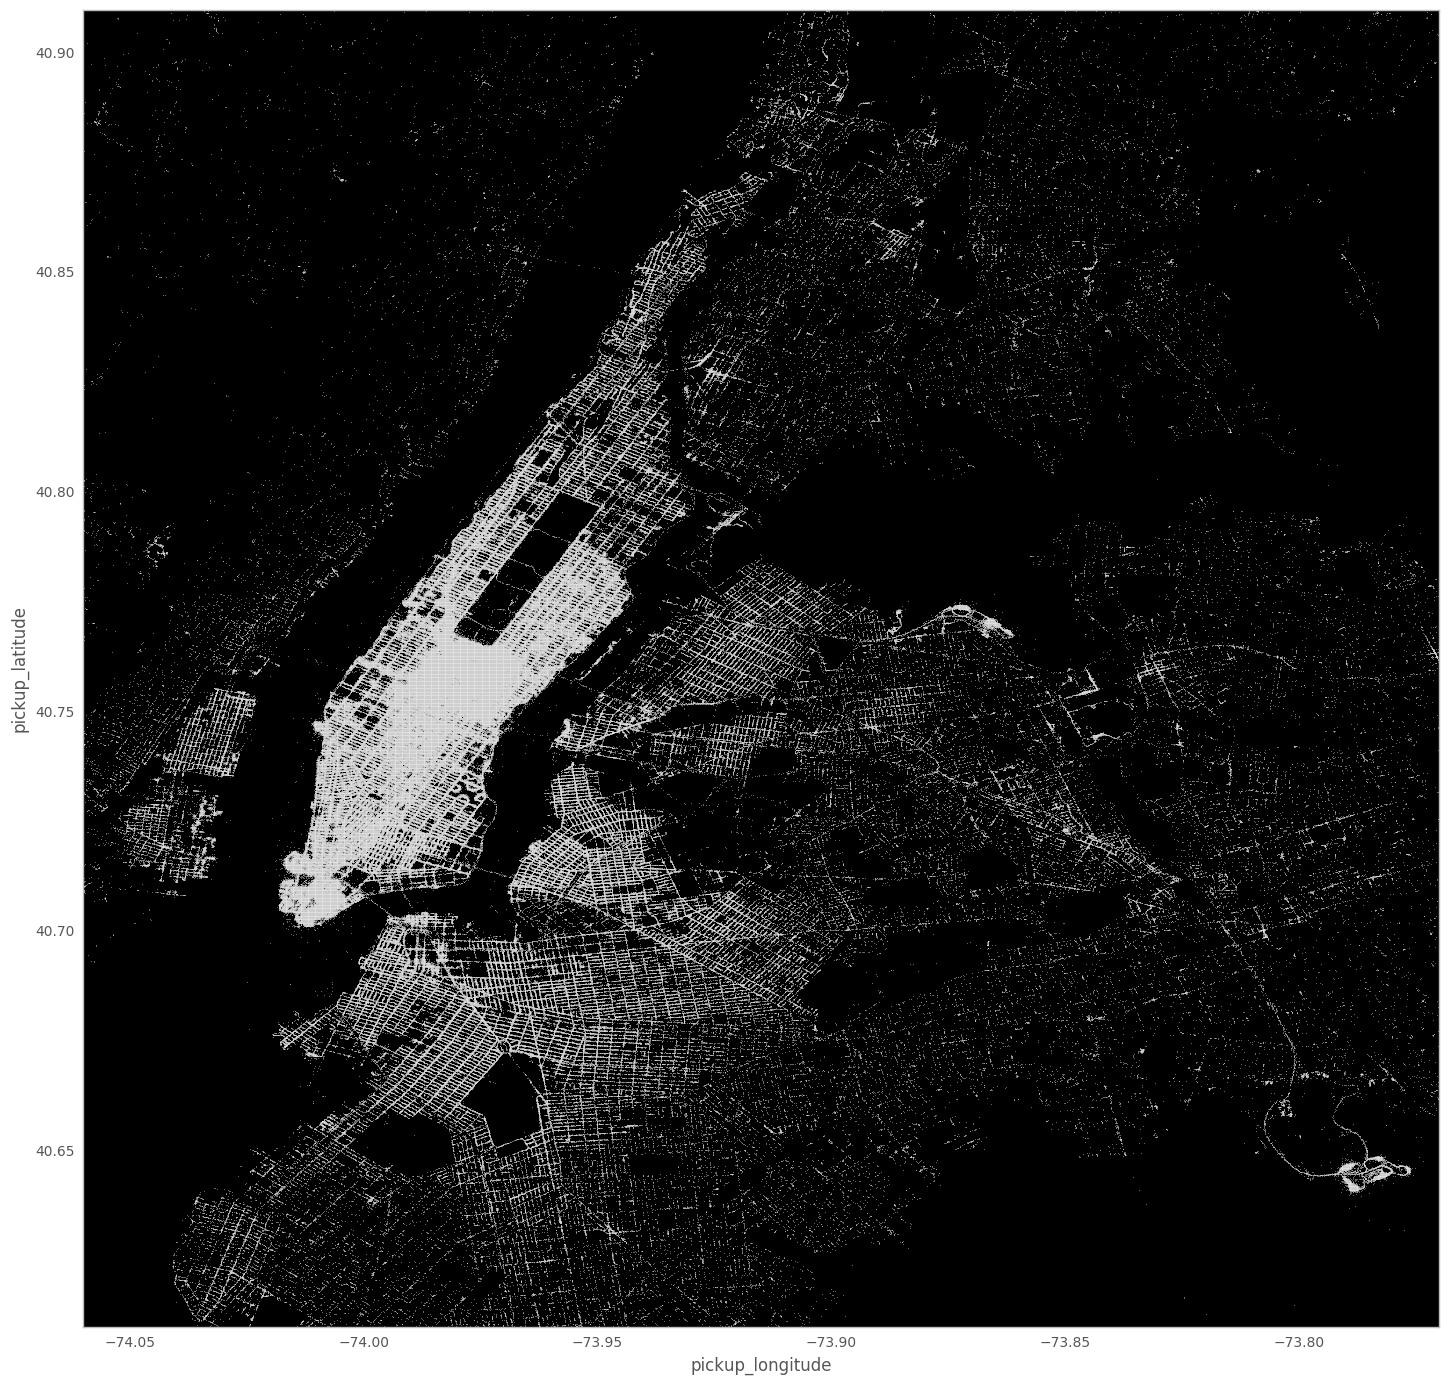
\includegraphics[width=\textwidth]{Complete.png}	

\break

\textbf{Milestone 2}

Following were the actions items decided for milestone 2
\begin{itemize}
	\item Binning
	\item Decide algorithmic approach for mining the pickup pattern
	\item Understanding GPFlow
\end{itemize}


\textbf{Binning  : }
The uber-dataset for all the 6 months contains around 4.5 millions records. Binning helps in reducing the number of the input required for model creation. Also it helped us in decided the label required for regression. 
Binning was done based on following creitera. \\
Time based binning : All the pickup rides are divided into 24 hours slot as per pickup time. \\
Location based binning : Entire NYC areas was divided into 'n' clusters. We used spatial DBSCAN for finding this each area center point.  \\

\textbf{Spatial DBSCAN:}


Kernel \\
\begin{center}
$K_{nm} = 1/\lambda \left ( \phi \phi ^{T} \right )$ \break

$\frac{1}{\lambda } \overrightarrow{\phi }\left ( \overrightarrow{X_{n}} \right )^{T}\overrightarrow{\phi }\left ( \overrightarrow{X_{m}} \right ) = \frac{1}{\lambda }l\left [ \overrightarrow{X_{n}},\overrightarrow{X_{m}} \right ]$ \break

$ K := \phi \phi ^{T}$ \break
s
\end{center}

As per Linear Rigression :: \\

\begin{center}
\(\theta\)   = $(XX^{T})^{-1}X^{T}Y$ 

\end{center}

Hence for Kernel Ridge Regression \\

\begin{center}

$E\left [w/y  \right ] =  A^{-1}\phi ^{T}Y$\ \break
                      
$A = (\phi^{T} \phi + \lambda I )$ \break

$\phi =  \phi \left ( X \right )$ \break

$K = 1/\lambda \left ( \phi \phi ^{T} \right )$ \break

$A^{-1}\phi ^{T} = \phi ^{T}\left ( K + \lambda I^{-1} \right )$ \break

$E\left [ f\left ( X\star  \right )/y \right ] = \phi \left ( x\star  \right )^{T}E\left [ w/y \right ]$

\end{center}
\end{document}